\documentclass[a4paper]{article}
\usepackage[utf8x]{inputenc}
\usepackage[T1,T2A]{fontenc}
\usepackage[russian]{babel}
\usepackage{hyperref}
\usepackage{indentfirst}
\usepackage{listings}
\usepackage{color}
\usepackage{here}
\usepackage{array}
\usepackage{multirow}
\usepackage{graphicx}
\usepackage{caption}
\graphicspath{{graphics/}}
\usepackage[left=2cm,right=2cm,
top=2cm,bottom=2cm,bindingoffset=0cm]{geometry}
\usepackage{listings}
\lstset{ %
	extendedchars=\true,
	keepspaces=true,
	language=bash,					% choose the language of the code
	basicstyle=\footnotesize,		% the size of the fonts that are used for the code
	numbers=left,					% where to put the line-numbers
	numberstyle=\footnotesize,		% the size of the fonts that are used for the line-numbers
	stepnumber=1,					% the step between two line-numbers. If it is 1 each line will be numbered
	numbersep=5pt,					% how far the line-numbers are from the code
	backgroundcolor=\color{white},	% choose the background color. You must add \usepackage{color}
	showspaces=false				% show spaces adding particular underscores
	showstringspaces=false,			% underline spaces within strings
	showtabs=false,					% show tabs within strings adding particular underscores
	frame=single,           		% adds a frame around the code
	tabsize=2,						% sets default tabsize to 2 spaces
	captionpos=b,					% sets the caption-position to bottom
	breaklines=true,				% sets automatic line breaking
	breakatwhitespace=false,		% sets if automatic breaks should only happen at whitespace
	escapeinside={\%*}{*)},			% if you want to add a comment within your code
	postbreak=\raisebox{0ex}[0ex][0ex]{\ensuremath{\color{red}\hookrightarrow\space}}
}

\begin{document}	% начало документа

\begin{titlepage}	% начало титульной страницы

	\begin{center}		% выравнивание по центру

		\large Санкт-Петербургский Политехнический Университет Петра Великого\\
		\large Институт компьютерных наук и технологий \\
		\large Кафедра компьютерных систем и программных технологий\\[6cm]
		% название института, затем отступ 6см
		
		\huge Телекоммуникационные технологии\\[0.5cm] % название работы, затем отступ 0,5см
		\large Отчет по лабораторной работе №5 \\[0.2cm]
		\large\textbf{"Частотная и фазовая модуляция"}\\[5cm]

	\end{center}


	\begin{flushright} % выравнивание по правому краю
		\begin{minipage}{0.25\textwidth} % врезка в половину ширины текста
			\begin{flushleft} % выровнять её содержимое по левому краю

				\large\textbf{Работу выполнила:}\\
				\large Власова А.В.\\
				\large {Группа:} 33501/4\\
				
				\large \textbf{Преподаватель:}\\
				\large Богач Н.В.\

			\end{flushleft}
		\end{minipage}
	\end{flushright}
	
	\vfill % заполнить всё доступное ниже пространство

	\begin{center}
	\large Санкт-Петербург\\
	\large \the\year % вывести дату
	\end{center} % закончить выравнивание по центру

\thispagestyle{empty} % не нумеровать страницу
\end{titlepage} % конец титульной страницы

\vfill % заполнить всё доступное ниже пространство

\section{Цель работы}
Изучение частотной и фазовой модуляции/демодуляции сигнала.

\section{Постановка задачи}
\begin{itemize}
	\item Сгенерировать однотональный сигнал низкой частоты.
	\item Выполнить фазовую модуляцию/демодуляцию сигнала по закону $u(t)=(U_mcos (\Omega t+ks(t))$, используя встроенную функцию MatLab pmmod, pmdemod
	\item Получить спектр модулированного сигнала.
	\item Выполнить частотную модуляцию/демодуляцию по закону
	
	$u(t)=U_mcos((\omega_0 t+k\int_{0}^{t}s(t)dt+\phi_0)$
	
	используя встроенные функции MatLab fmmod, fmdemod
\end{itemize}


\section{Теоретический раздел}
Частотная модуляция — вид аналоговой модуляции, при котором информационный сигнал управляет частотой несущего колебания. По сравнению с амплитудной модуляцией здесь амплитуда остаётся постоянной. 

Фазовая модуляция - модуляция, при которой фаза несущей изменяется прямо пропорционально информационному сигналу. В реальности чаще применяеют термин фазовая манипуляция, т.к. в основном производят манипуляцию дискретных сигналов.
 
\section{Ход работы}
Сгенерируем однотональный сигнал низкой частоты.
\captionof{lstlisting}{Генерация модулирующего сигнала}
\lstinputlisting[firstline=4, lastline=13]{../lab5.m}
\begin{center}
	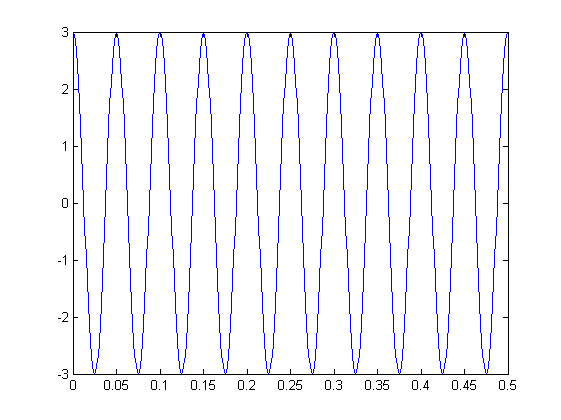
\includegraphics[scale = 0.7]{sign.png} \\Рис.1 Модулирующий сигнал
\end{center}

Выполним фазовую модуляцию, используя функцию pmmod.
\captionof{lstlisting}{Фазовая модуляция}
\lstinputlisting[firstline=15, lastline=21]{../lab5.m}
\begin{center}
	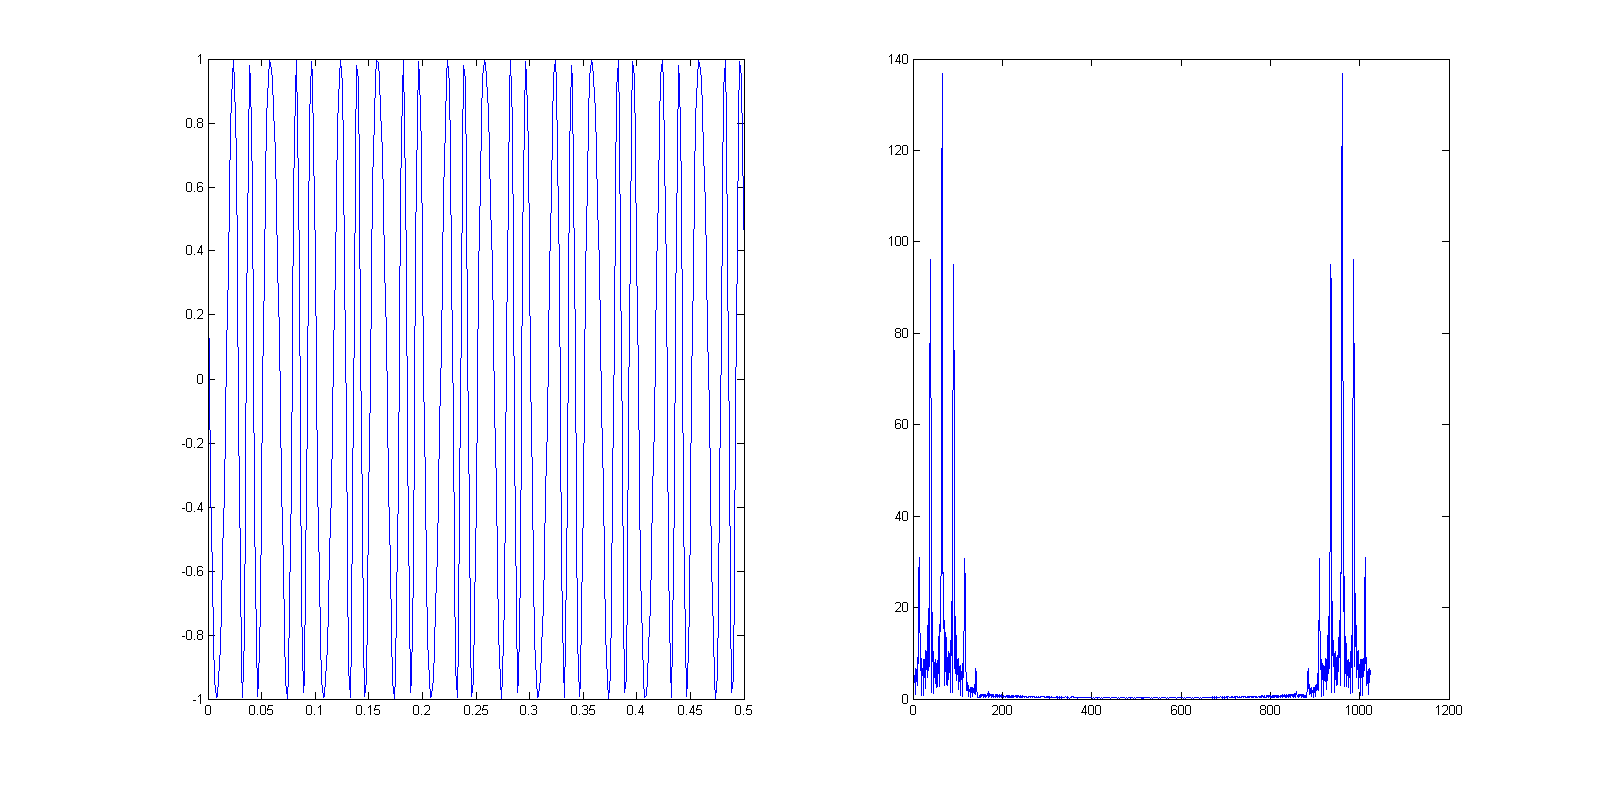
\includegraphics[scale = 0.45]{pm.png} \\Рис.2 Фазовая модуляция
\end{center}

Выполним демодуляцию ФМ-сигнала.
\captionof{lstlisting}{Демодуляция ФМ-сигнала}
\lstinputlisting[firstline=23, lastline=28]{../lab5.m}
\begin{center}
	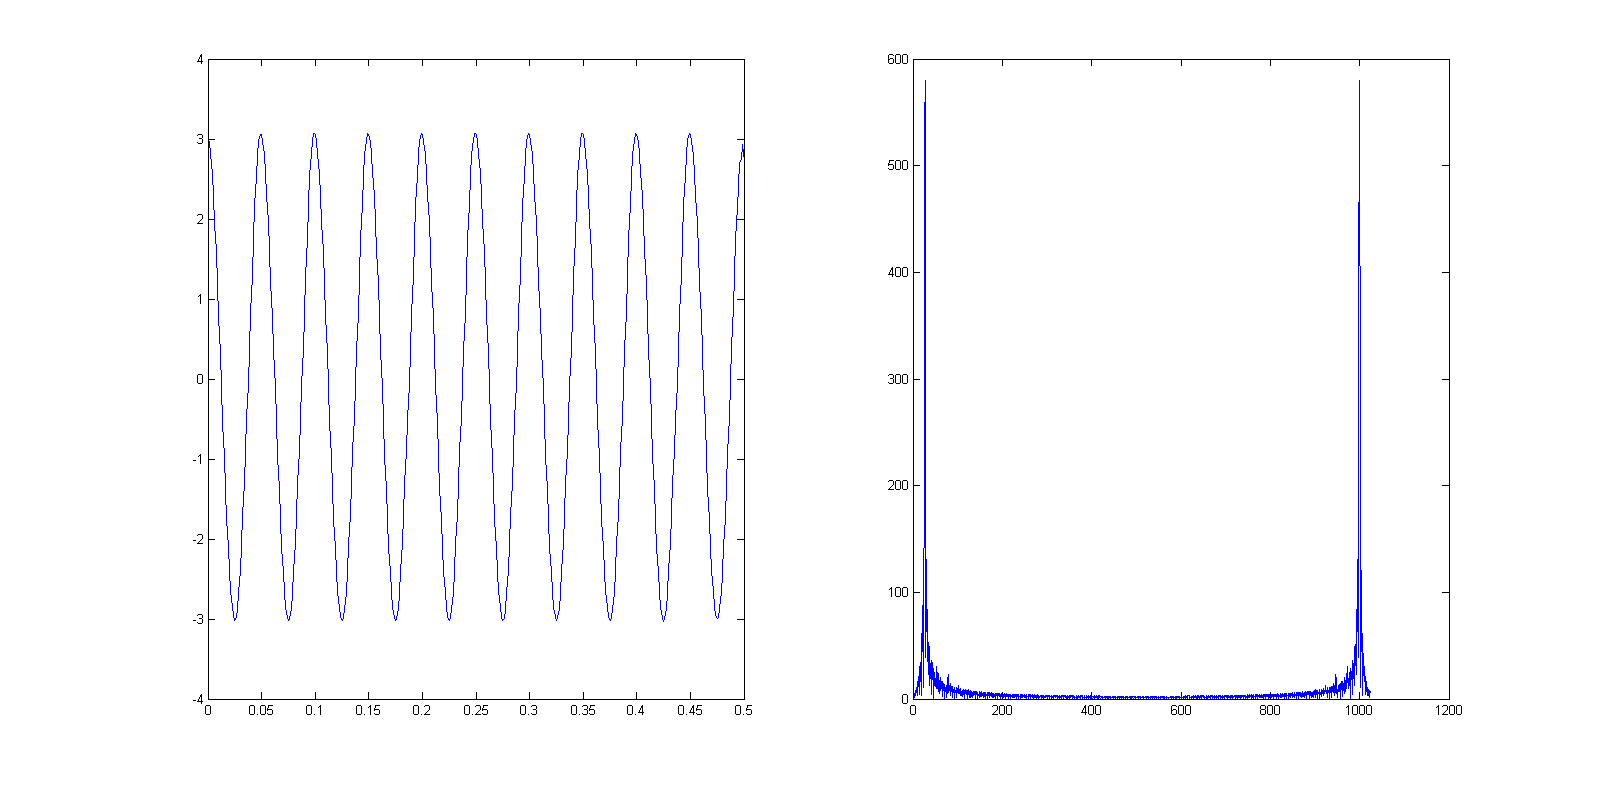
\includegraphics[scale = 0.45]{pm_demod.png} \\Рис.3 Демодуляция ФМ-сигнала
\end{center}

Выполним частотную модуляцию, используя функцию fmmod.
\captionof{lstlisting}{Частотная модуляция}
\lstinputlisting[firstline=30, lastline=36]{../lab5.m}
\begin{center}
	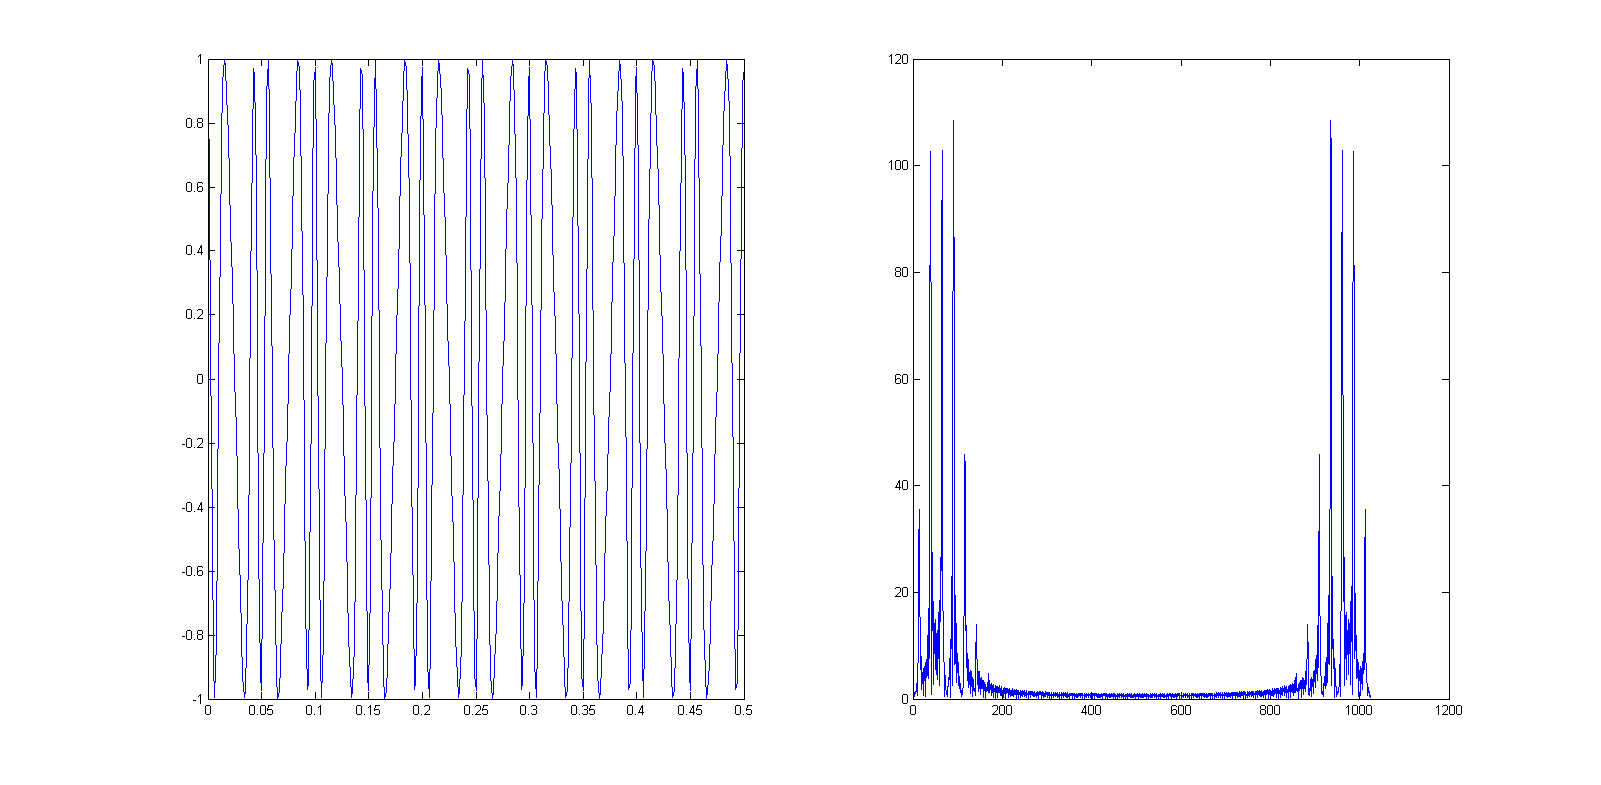
\includegraphics[scale = 0.45]{fm.png} \\Рис.4 Частотная модуляция
\end{center}

Выполним демодуляцию ЧМ-сигнала.
\captionof{lstlisting}{Демодуляция ЧМ-сигнала}
\lstinputlisting[firstline=38, lastline=45]{../lab5.m}
\begin{center}
	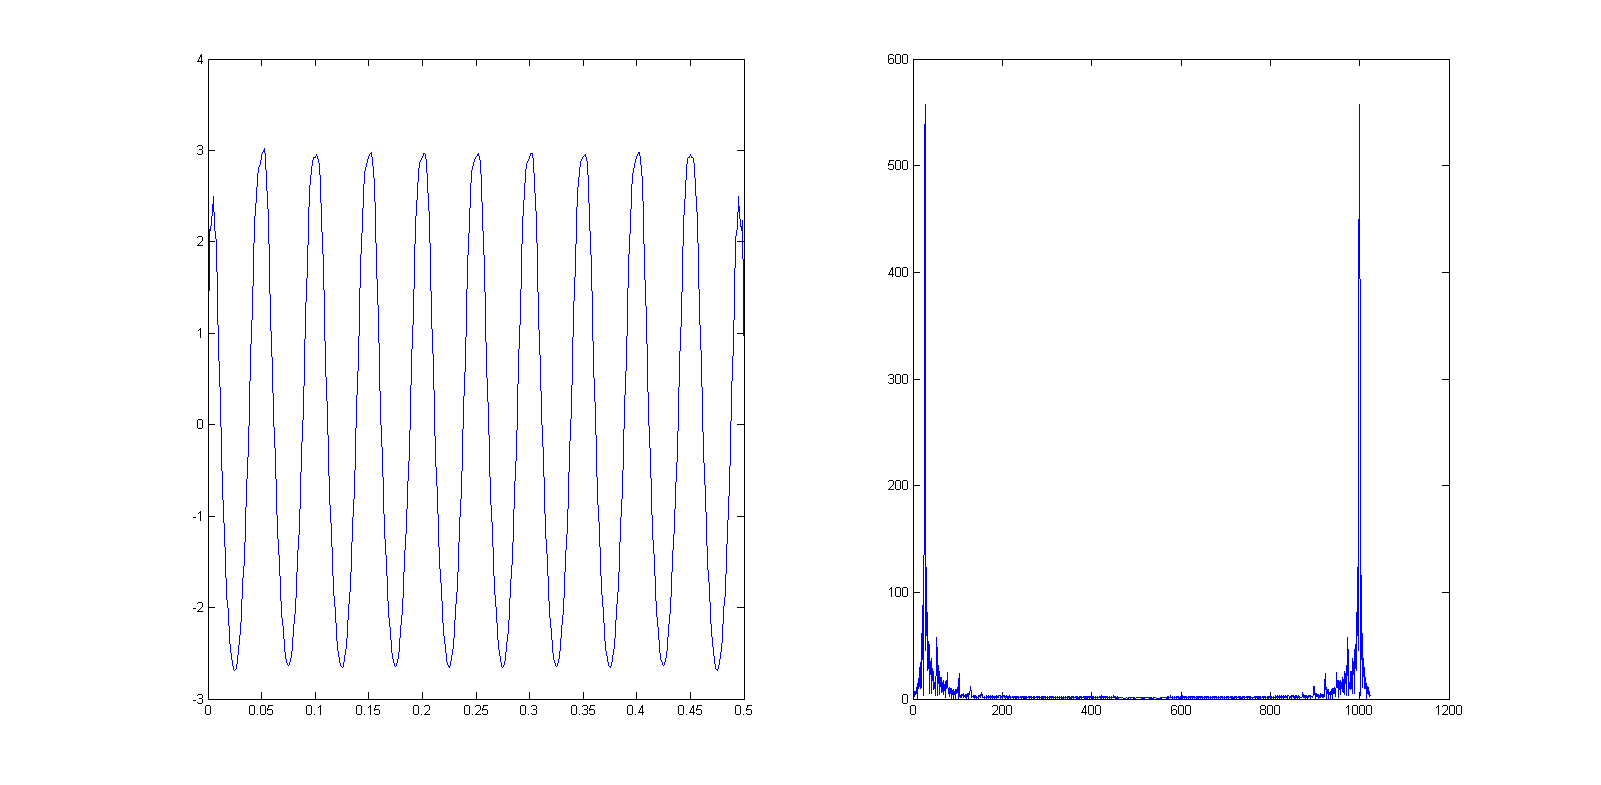
\includegraphics[scale = 0.45]{fm_demod.png} \\Рис.5 Думодуляция ЧМ-сигнала
\end{center}



\section{Выводы}
В ходе выполнения лабораторной работы исследована фазовая и частотная модуляция/демодуляция сигналов. Модуляция сигналов находит широкое применение в телекоммуникационных технологиях. Так, например, частотная модуляция используется для высококачественной передачи звукового сигнала в теле- и радиовещании, в сотовой телефонной связи и других системах. 
\end{document}



